\documentclass[11pt]{article}
\usepackage{ucs}
\usepackage[utf8x]{inputenc}
\usepackage{changepage}
\usepackage{graphicx}
\usepackage{amsmath}
\usepackage{gensymb}
\usepackage{amssymb}
\usepackage{enumerate}
\usepackage{tabularx}
\usepackage{lipsum}
\usepackage{hyperref}

\oddsidemargin 0.0in
\evensidemargin 0.0in
\textwidth 6.27in
\headheight 1.0in
\topmargin -0.1in
\headheight 0.0in
\headsep 0.0in
\textheight 9.0in

\setlength\parindent{0pt}

\newenvironment{myenv}{\begin{adjustwidth}{0.4in}{0.4in}}{\end{adjustwidth}}
\renewcommand{\abstractname}{Anotācija}
\renewcommand\refname{Atsauces}



\newcounter{alphnum}
\newenvironment{alphlist}{\begin{list}{(\Alph{alphnum})}{\usecounter{alphnum}\setlength{\leftmargin}{2.5em}} \rm}{\end{list}}

\makeatletter
\let\saved@bibitem\@bibitem
\makeatother

\usepackage{bibentry}
%\usepackage{hyperref}


\begin{document}

\thispagestyle{empty}

{\Large Lietišķie algoritmi \textendash{} Semestra vidus eksāmens jeb ``Midterm'' (2019-10-29)}

\noindent
{\bf 1.uzdevums (1+1+1+2 punkti):}
Spēlētājs $X$ vienā gājienā izņem no urnas trīs kartiņas. 
Pieņemsim, ka urna ir ļoti liela, kartiņas tajā nekad nebeidzas un ir vienādas varbūtības
izķeksēt jebkuru no burtiem {\tt A}, {\tt B} vai {\tt C}; citu burtu urnā nav.
Pēc tam $X$ sakārto trīs kartiņas alfabētiskā secībā un nosūta spēlētājam $Y$ ziņojumu \textendash{} to burtu, kurš 
pēc sakārtošanas bija pirmais. (Piemēram, ja izķeksētie burti ir {\tt "CBC"}, tad pēc sakārtošanas tie būs {\tt "BCC"} un 
$X$ nosūta ziņojumu {\tt "B"}.) 
\begin{enumerate}[(a)]
\item Kāds ir informācijas saturs ziņojumam {\tt A}?
\item Kāds ir informācijas saturs ziņojumam {\tt B}? 
\item Kāds ir informācijas saturs ziņojumam {\tt C}? 
\item Kāda ir entropija jebkuram vienam ziņojumam, ko $X$ nosūta $Y$ saskaņā ar augšminēto procedūru?
\end{enumerate}

\vspace{6pt}
\noindent
{\bf 2.uzdevums (3 punkti - jebkāds pareizs Hafmana koks, 3 punkti - koks kanoniskajā formā):}
Hafmana koku sauksim par {\em kanonisku}, ja izpildās sekojošas īpašības: 
\begin{itemize}
\item Visi kanoniskā koka zari (ceļi no saknes līdz lapām/ziņojumiem) veido garumus, kuri ir nedilstošā secībā, skaitot no augšas uz leju.
\item Vienāda garuma zariem ziņojumi izkārtoti ziņojumu alfabētiskā secībā. 
\end{itemize}
Attēla 1.piemērā zaru garumi nav nedilstošā secībā
(zars $\mathtt{11}$ uz lapu $\mathtt{A}$ ir garumā $2$, virs tā divi zari garumā $3$). 
2.piemērā $\mathtt{C}$, $\mathtt{D}$ ir ar vienādi gariem kodavārdiem, bet nav alfabētiskā secībā.\\
Vienīgi 3.piemērā Hafmana koks ir kanonisks.

\begin{center}
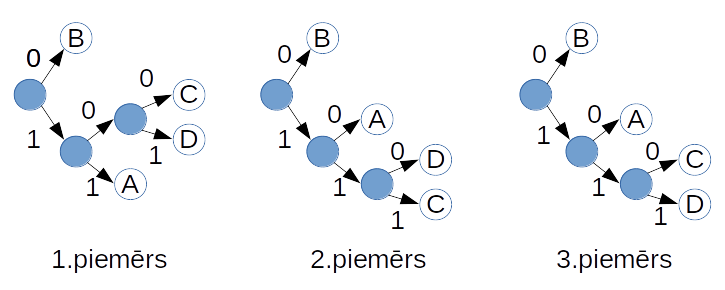
\includegraphics[width=0.5\textwidth]{huffman-examples.png}
\end{center}

$5$ ziņojumu kopai $\{ \mathtt{A},\mathtt{B},\mathtt{C},\mathtt{D},\mathtt{E} \}$, kuru varbūtības ir attiecīgi 
${\displaystyle \left\{ \frac{1}{15}, \frac{2}{15},\frac{3}{15},\frac{4}{15},\frac{5}{15} \right\}}$,
atrast un uzzīmēt kanonisku Hafmana koku.


\vspace{6pt}
{\bf 3.uzdevums (4 punkti):}
Izmantojot LZ78 algoritmu 6 simbolu alfabētam $\{\mathtt{C}, \mathtt{E}, \mathtt{L}, \mathtt{N},\mathtt{S}, \mathtt{U}\}$,
izveidot tabulu un nokodēt sekojošu $15$ simbolu ziņojumu: {\tt SUCCESSLESSNESS}. 
Tabulā attēlot soļa numuru, $w$ - garāko vārdnīcā jau atrodamo simbolu virkni, $k$ - virknei $w$ sekojošo simbolu, algoritma izvadi un 
vārdnīcai attiecīgajā solī pievienojamo vārdu. 

\begin{center}
\begin{tabular}{ |l|l|l|l|l| } \hline
Solis & $w$ & $k$ & Izvade & Pievieno vārdnīcai \\ \hline
$\ldots$ & $\ldots$ & $\ldots$ & $\ldots$ & $\ldots$ \\ \hline
\end{tabular}
\end{center}


\vspace{6pt}
{\bf 4.uzdevums (6 punkti):}
Veikt inverso Berouza-Vīlera transformāciju $17$ simbolu virknītei: {\tt SETTNRSDDIESIEESN}, 
ja zināms, ka kodētais vārds ir pats pirmais starp leksikogrāfiski sakārtotajām cikliskajām permutācijām. 


\vspace{6pt}
{\bf 5.uzdevums (2+3 punkti):} 
Kvantizācijas algoritms saņem ieejā attēla krāsu intensitātes, kuras ir veseli skaitļi 
$x \in \{ 0, 1,2,\ldots,255 \}$ un atgriež apakšējo veselo daļu: ${\displaystyle \left\lfloor \frac{x}{10} \right\rfloor}$
jeb nomet tā decimālpieraksta pēdējo ciparu. 
\begin{enumerate}[(a)]
\item 
Ja visas šīs kvantizētās vērtības būtu jāsūta, izmantojot vienādu, fiksētu bitu skaitu \textendash{} cik lielu saspiešanas 
attiecību ({\em compression ratio} \textendash{} sākotnējā faila izmēra attiecību pret saspiestā faila izmēru) varētu sasniegt?
\item
Pieņemot, ka visas krāsu intensitātes (no $0$ līdz $255$) ir ar vienādām varbūtībām, 
kāda ir jaunās, kvantizētās ziņojumu virknes entropija? Kāda būtu teorētiski labākā iespējamā saspiešanas attiecība (ja izmantotu
aritmētisko kodējumu vai citu optimālu metodi, kas tuvojas entropijas noteiktajai saspiešanas robežai).
\end{enumerate}


\vspace{6pt}
{\bf 6.uzdevums (4 punkti):}
Spēlētājs $X$ vēlas nosūtīt spēlētājam $Y$ dažus ceturtās pakāpes polinomus ar veseliem koeficientiem: 
$$f(x) = a_0x^4 + a_1x^3 + a_2x^2 + a_3x + a_4,\;\;\text{kur}\;\;a_0,\ldots,a_4 \in \mathbb{Z}.$$
Polinoma koeficientu $a_i$ vietā spēlētājs $X$ sūta $s$ vērtības dažādiem veseliem argumentiem: 
$$f(0),f(1),\ldots,f(s-1).$$
Vidū starp spēlētājiem $X$ un $Y$ atrodas ļaunprātīgais Šlopsterklopsters, kurš ne vairāk kā piecas
no visām $s$ nosūtītajām vērtībām drīkst nomainīt ar citiem skaitļiem (bet drīkst nomainīt arī mazāku skaitu 
vērtību vai nenomainīt nevienu).\\
Uzrakstīt nevienādību attiecībā pret parametru $s$ (un atrisināt to), lai uzzinātu mazāko polinoma vērtību skaitu $s$, kuram
spēlētājs $Y$ noteikti varēs atjaunot $X$'a sūtīto polinomu, lai kā arī nerīkotos Šlopsterklopsters.



\vspace{6pt}
{\bf 7.uzdevums (2+2+2 punkti):} 
(Ieteikums: Šajā uzdevumā var izmantot algebriskas identitātes par skaitļu kāpināšanu, Eilera teorēmu u.c. skaitļu teorijas rezultātus.)
\begin{enumerate}[(a)]
\item Kriptogrāfijas algoritmam ir jāaprēķina $4^{143}\;(\text{mod}\,199)$ (atlikums, kas rodas dalot $4^{139}$ ar $199$). 
Algoritms var ielūkoties reizināšanas tabulā pēc moduļa $199$: ievadīt divus skaitļus $a,b$ un saņemt to reizinājumu 
$a\cdot{}b\;(\text{mod}\,199)$ ($ab$ atlikumu, dalot ar $199$).
Kādu mazāko reižu skaitu pietiek ielūkoties reizināšanas tabulā, lai atrastu $4^{139}\;(\text{mod}\,199)$.\\
{\em Piezīme.} Algoritms var veikt arī dalīšanu ar atlikumu un atņemšanu, bet jāsaskaita tikai reizināšanas darbības.
(Acīmredzot, pietiek veikt $142$ reizināšanas; Jūsu uzdevums ir reizināšanu skaitu pēc iespējas samazināt.)
\item Kriptogrāfijas algoritmam ir jāaprēķina $4^{143}\;(\text{mod}\,7)$. Algoritms var ielūkoties reizināšanas tabulā 
pēc moduļa $7$. Kādu mazāko reizināšanu skaitu vajag, lai atrastu rezultātu? 
\item Atrast $4^{143}\;(\text{mod}\,7)$ vērtību; parādīt, kā tā iegūta.
\end{enumerate}



\end{document}



